% ===================== CHAPITRE 3 : CONCEPTION ET MODÉLISATION =====================

\section*{Introduction}
Ce chapitre constitue le cœur du travail~: architecture logique du système,
modélisation dynamique (séquence, activité), modélisation statique (classes) et
conception de la base de données (MCD, MLD, dictionnaire de données, règles de
gestion, normalisation).

\section{Architecture logique du système}
\label{sec:archi-logicielle}

Le système est conçu en couches, séparant la présentation, la logique
applicative et la persistance.

\begin{table}[H]
\centering
\renewcommand{\arraystretch}{1.25}
\begin{tabularx}{\linewidth}{>{\bfseries}p{3.2cm} X}
\toprule
Couche & Responsabilités \\
\midrule
Présentation      & Rendu des vues, carte interactive, formulaires, navigation. \\
Application (API) & Accès aux ressources, validation, contrôle d'accès par rôle, règles métier. \\
Accès aux données & Correspondance objets $\leftrightarrow$ tables, requêtes, transactions. \\
Persistance (SGBD) & Stockage relationnel, intégrité référentielle, index. \\
Services externes & Fond de carte et géocodage (OpenStreetMap). \\
\bottomrule
\end{tabularx}
\caption{Découpage en couches}
\label{tab:couches}
\end{table}

Les ressources manipulées sont~: \emph{utilisateurs}, \emph{annonces},
\emph{biens} (localisation), \emph{images}, \emph{référentiel géographique}
(gouvernorat, délégation, localité), \emph{favoris}, \emph{recherches
sauvegardées}. Le référentiel géographique est exposé sous forme de listes
dépendantes~: les délégations d'un gouvernorat, puis les localités d'une
délégation, avec une recherche textuelle de lieu retournant le niveau trouvé et
ses parents.

\section{Modélisation dynamique}
\label{sec:dynamique}

\subsection{Diagramme de séquence : recherche cartographique}
\begin{figure}[H]
  \centering
  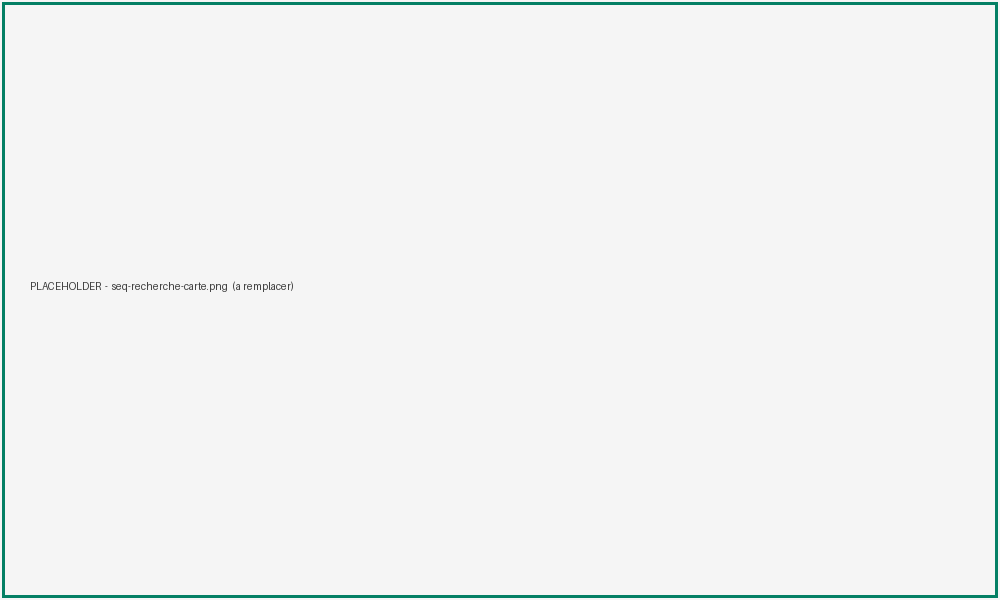
\includegraphics[width=0.9\linewidth]{images/seq-recherche-carte.png} % À FOURNIR
  \caption{Séquence « Rechercher un bien sur la carte »}
  \label{fig:seq-recherche}
\end{figure}
\noindent Le client transmet l'emprise courante de la carte~; le système renvoie
les biens dont les coordonnées appartiennent à cette emprise et dont l'annonce
est approuvée~; le client place les marqueurs et applique le regroupement.

\subsection{Diagramme de séquence : publication d'une annonce géolocalisée}
\begin{figure}[H]
  \centering
  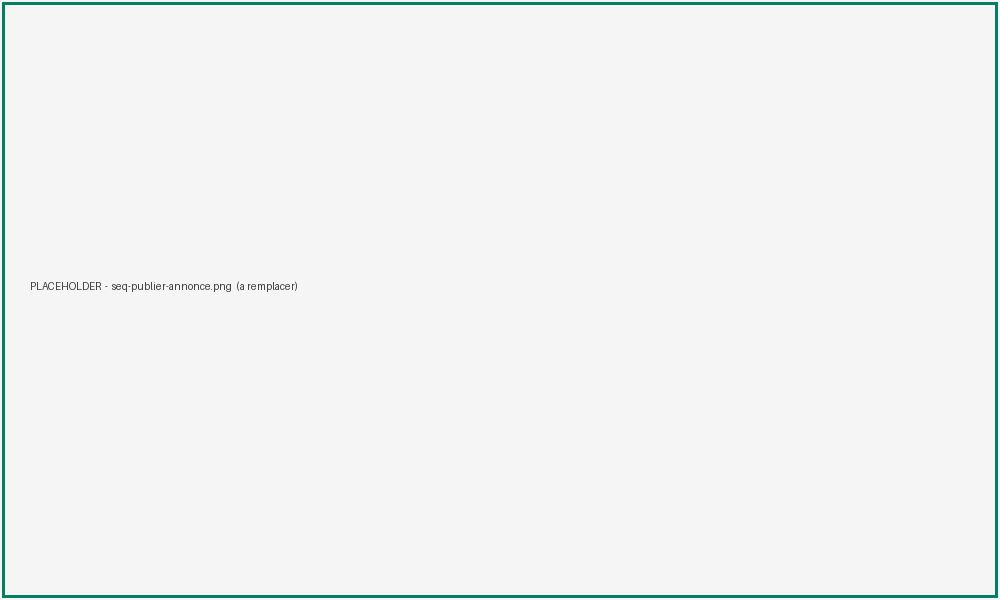
\includegraphics[width=0.9\linewidth]{images/seq-publier-annonce.png} % À FOURNIR
  \caption{Séquence « Publier une annonce géolocalisée »}
  \label{fig:seq-publier}
\end{figure}
\noindent Points remarquables~: (i) au dépôt du marqueur, un \textbf{géocodage
inverse} propose une adresse~; (ii) à la soumission, le système crée
l'\texttt{Annonce}, le \texttt{Bien} associé (relation 1--1) et ses images~;
(iii) l'annonce est créée à l'état \texttt{en attente}.

\subsection{Diagramme d'activité : cycle de vie d'une annonce}
\begin{figure}[H]
  \centering
  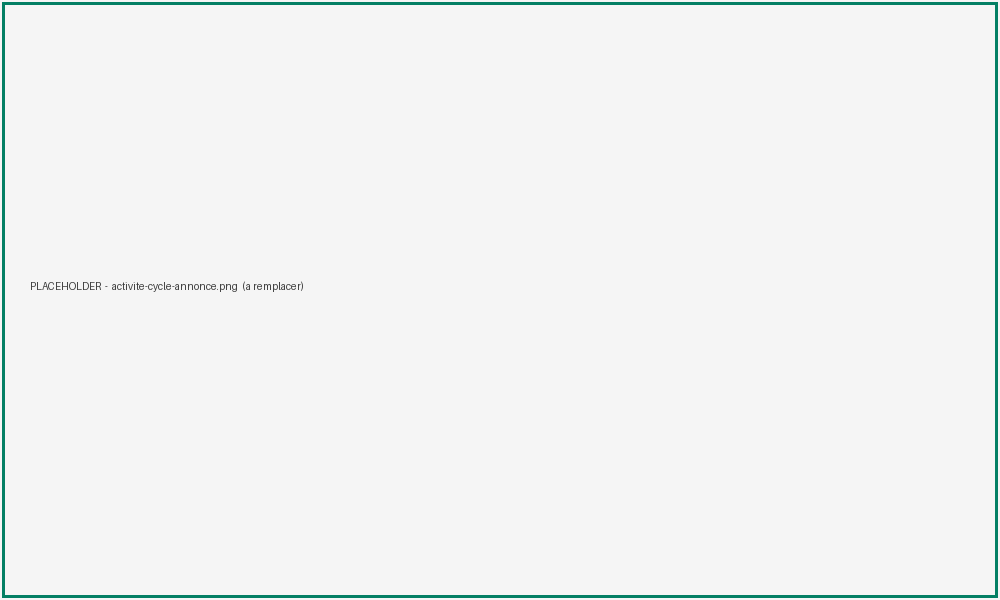
\includegraphics[width=0.62\linewidth]{images/activite-cycle-annonce.png} % À FOURNIR
  \caption{Cycle de vie d'une annonce (en attente, approuvée, refusée, vendue, louée)}
  \label{fig:cycle-annonce}
\end{figure}

\section{Modélisation statique : diagramme de classes}
\label{sec:classes}

\begin{figure}[H]
  \centering
  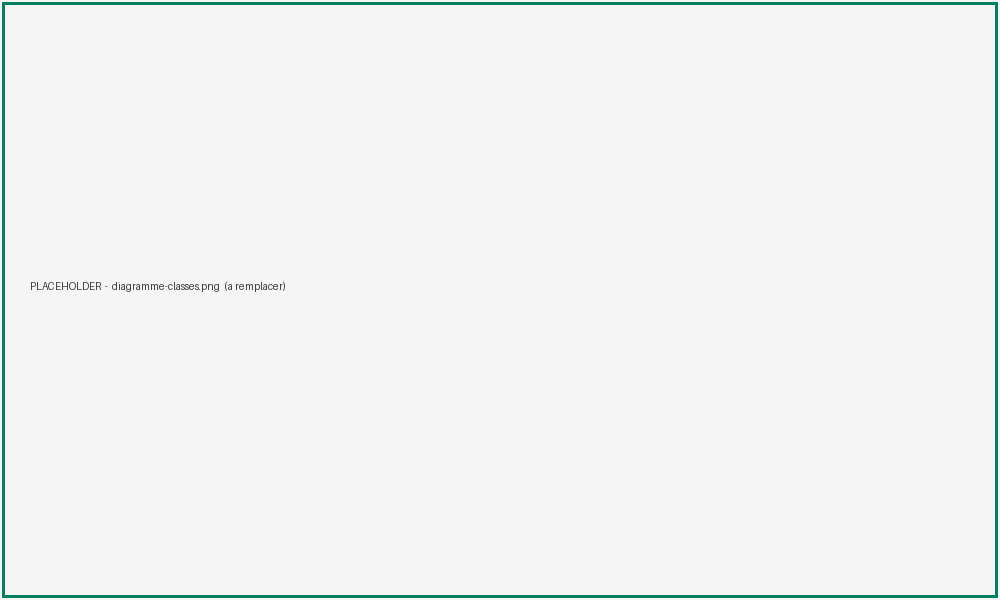
\includegraphics[width=\linewidth]{images/diagramme-classes.png} % À FOURNIR
  \caption{Diagramme de classes du domaine}
  \label{fig:classes}
\end{figure}

\begin{table}[H]
\centering
\renewcommand{\arraystretch}{1.2}
\begin{tabularx}{\linewidth}{>{\bfseries}p{3.1cm} X}
\toprule
Classe & Rôle \\
\midrule
\texttt{Utilisateur} & Compte de la plateforme~; porte le rôle (particulier, agent, agence, promoteur, administrateur) et le profil. \\
\texttt{Agence}       & Entité professionnelle rattachée à un utilisateur~; regroupe des agents. \\
\texttt{Annonce}      & Offre de vente / location / vacances d'un bien~; porte l'état de modération, le prix, les caractéristiques générales. \\
\texttt{Bien}         & Localisation~: adresse, latitude, longitude, image principale~; relation 1--1 avec \texttt{Annonce}. \\
\texttt{Image}        & Photo d'un bien, avec un ordre d'affichage. \\
\texttt{Gouvernorat}, \texttt{Delegation}, \texttt{Localite} & Référentiel géographique hiérarchique. \\
\texttt{Favori}       & Association \texttt{Utilisateur}--\texttt{Annonce} (bien enregistré). \\
\texttt{RechercheSauvegardee} & Critères de recherche d'un utilisateur + alerte. \\
\bottomrule
\end{tabularx}
\caption{Classes principales du modèle}
\label{tab:classes-principales}
\end{table}

\paragraph{Associations et multiplicités.}
\begin{itemize}[label=\textbullet,itemsep=1pt]
  \item \texttt{Utilisateur} \emph{1} --- \emph{0..*} \texttt{Annonce}~;
  \item \texttt{Annonce} \emph{1} --- \emph{1} \texttt{Bien}~;
        \texttt{Bien} \emph{1} --- \emph{0..*} \texttt{Image}~;
  \item \texttt{Gouvernorat} \emph{1} --- \emph{0..*} \texttt{Delegation}
        \emph{1} --- \emph{0..*} \texttt{Localite}~;
  \item \texttt{Annonce} \emph{*} --- \emph{1} de chacun de
        \texttt{Gouvernorat}, \texttt{Delegation}, \texttt{Localite}~;
  \item \texttt{Utilisateur} \emph{*} --- \emph{*} \texttt{Annonce} via
        \texttt{Favori}~;
  \item \texttt{Agence} \emph{1} --- \emph{0..*} \texttt{Utilisateur} (agents).
\end{itemize}

\paragraph{Énumérations du domaine.}
\begin{table}[H]
\centering
\renewcommand{\arraystretch}{1.15}
\begin{tabularx}{\linewidth}{>{\bfseries}p{3cm} X}
\toprule
Énumération & Valeurs (extrait) \\
\midrule
Rôle          & admin, promoteur, agence, agent, particulier \\
Catégorie     & vente, location, vacances \\
Type de bien  & appartement, duplex, penthouse, villa, bureau, local commercial, terrain, ferme agricole, immeuble, garage/parking \\
État du bien  & nouveau, bon état, à rénover, en cours de construction \\
Statut d'annonce & en attente, approuvée, refusée, vendue, louée \\
Devise        & DT, EUR, USD \\
\bottomrule
\end{tabularx}
\caption{Principales énumérations}
\label{tab:enums}
\end{table}

\section{Conception de la base de données}
\label{sec:bdd}

\subsection{Choix du SGBD}
Le choix se porte sur un SGBD \textbf{relationnel} (PostgreSQL) pour l'intégrité
référentielle et le typage riche (numérique décimal pour les prix, énumérations,
dates), avec la possibilité d'une extension spatiale (PostGIS) si des requêtes
géographiques avancées (recherche par rayon, distance) deviennent nécessaires.

\subsection{Modèle conceptuel de données (MCD)}
\begin{figure}[H]
  \centering
  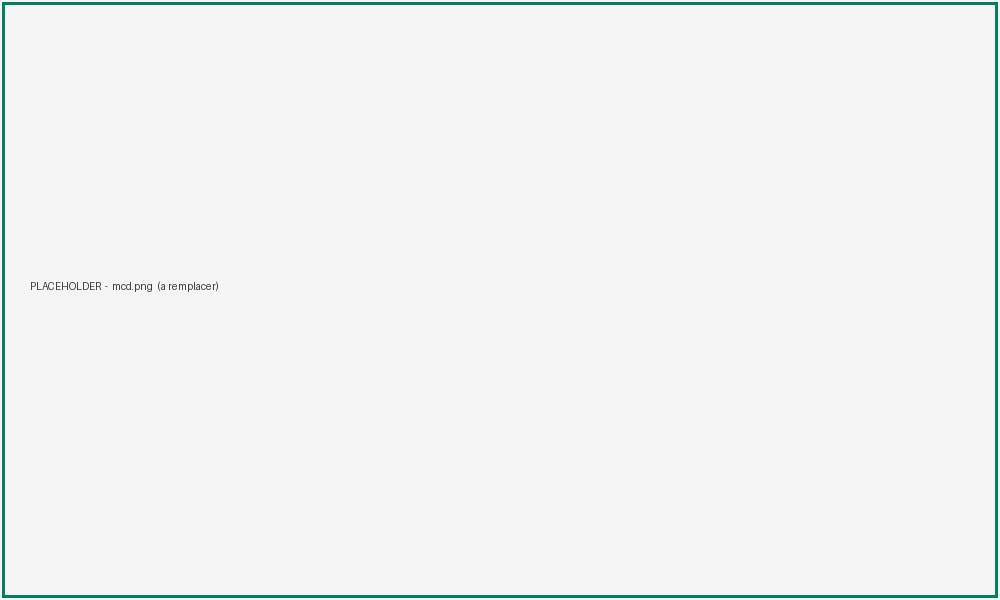
\includegraphics[width=\linewidth]{images/mcd.png} % À FOURNIR (Looping / draw.io)
  \caption{Modèle conceptuel de données}
  \label{fig:mcd}
\end{figure}
\noindent Le triplet géographique modélise une hiérarchie stricte sans cycle~;
l'entité \textsc{Bien} porte les coordonnées~; l'adresse administrative d'une
annonce est \emph{référencée} et non dupliquée.

\subsection{Modèle logique de données (MLD)}
Clés primaires soulignées, clés étrangères en italique.

\begin{longtable}{p{3.2cm} p{10.3cm}}
\caption{Modèle logique de données (extrait)}\label{tab:mld}\\
\toprule
\textbf{Relation} & \textbf{Attributs} \\
\midrule
\endfirsthead
\toprule
\textbf{Relation} & \textbf{Attributs} \\
\midrule
\endhead
users        & \underline{id}, username, email, mot\_de\_passe, role, telephone, nom, prenom, nom\_entreprise, \textit{agence\_id}, gouvernorat, localite, date\_creation \\
agencies     & \underline{id}, \textit{user\_id}, nom, email, telephone, adresse, matricule, reference, date\_creation \\
gouvernorats & \underline{id}, nom \\
delegations  & \underline{id}, nom, \textit{gouvernorat\_id} \\
localites    & \underline{id}, nom, \textit{delegation\_id} \\
annonces     & \underline{id}, reference, \textit{utilisateur\_id}, \textit{gouvernorat\_id}, \textit{delegation\_id}, \textit{localite\_id}, categorie, type\_bien, etat\_bien, titre, description, superficie, prix, devise, status, nb\_pieces, nb\_chambres, nb\_salles\_bain, date\_creation, date\_mise\_a\_jour \\
biens        & \underline{id}, \textit{annonce\_id} (unique), adresse, latitude, longitude, image\_principale \\
images       & \underline{id}, \textit{bien\_id}, url, ordre \\
favoris      & \underline{id}, \textit{user\_id}, \textit{annonce\_id}, date \; -- \; UNIQUE(user\_id, annonce\_id) \\
recherches\_sauvegardees & \underline{id}, \textit{user\_id}, nom, criteres, alerte\_email, date \\
\bottomrule
\end{longtable}

\subsection{Dictionnaire de données}
\begin{longtable}{p{2.8cm} p{2.5cm} p{2cm} p{5.4cm}}
\caption{Dictionnaire de données (tables centrales)}\label{tab:dictionnaire}\\
\toprule
\textbf{Attribut} & \textbf{Type} & \textbf{Contraintes} & \textbf{Description} \\
\midrule
\endfirsthead
\toprule
\textbf{Attribut} & \textbf{Type} & \textbf{Contraintes} & \textbf{Description} \\
\midrule
\endhead
\multicolumn{4}{l}{\textit{Table \texttt{annonces}}}\\
id            & entier        & PK, auto       & Identifiant annonce \\
reference     & chaîne        & unique         & Référence lisible (ex. TN0001) \\
utilisateur\_id & entier      & FK users.id    & Auteur de l'annonce \\
gouvernorat\_id & entier      & FK             & Gouvernorat \\
delegation\_id & entier       & FK             & Délégation \\
localite\_id  & entier        & FK             & Localité \\
categorie     & énum          & non nul        & vente / location / vacances \\
type\_bien    & énum          & non nul        & Type de bien \\
etat\_bien    & énum          &                & État du bien \\
titre         & chaîne        & non nul        & Titre de l'annonce \\
superficie    & réel          &                & Surface en m\textsuperscript{2} \\
prix          & décimal(12,2) & $>$ 0          & Prix \\
devise        & énum          & défaut DT      & Devise \\
status        & énum          & défaut en attente & État de modération \\
date\_creation & horodatage   & défaut \emph{now} & Date de dépôt \\
\midrule
\multicolumn{4}{l}{\textit{Table \texttt{biens}}}\\
id            & entier        & PK, auto       & Identifiant du bien \\
annonce\_id   & entier        & FK, \textbf{unique} & Annonce associée (1--1) \\
adresse       & chaîne        &                & Adresse lisible (géocodage inverse) \\
latitude      & réel          &                & Latitude WGS 84 (degrés décimaux) \\
longitude     & réel          &                & Longitude WGS 84 (degrés décimaux) \\
image\_principale & chaîne    & nullable       & URL de l'aperçu \\
\midrule
\multicolumn{4}{l}{\textit{Tables \texttt{gouvernorats} / \texttt{delegations} / \texttt{localites}}}\\
id            & entier        & PK, auto       & Identifiant \\
nom           & chaîne        & non nul        & Libellé \\
gouvernorat\_id & entier      & FK (delegations) & Gouvernorat parent \\
delegation\_id & entier       & FK (localites)  & Délégation parente \\
\bottomrule
\end{longtable}

\subsection{Règles de gestion}
\begin{enumerate}[label=RG-\arabic*.,itemsep=1pt]
  \item Une annonce appartient à un et un seul utilisateur.
  \item Une annonce décrit exactement un bien, et réciproquement (relation 1--1
        garantie par l'unicité de \texttt{annonce\_id} dans \texttt{biens}).
  \item Une localité appartient à une délégation, une délégation à un
        gouvernorat~; la hiérarchie ne comporte pas de cycle.
  \item Le triplet (gouvernorat, délégation, localité) d'une annonce est
        cohérent avec la hiérarchie.
  \item Les coordonnées doivent être situées dans l'emprise de la Tunisie
        (contrôle applicatif).
  \item Une annonce est créée à l'état « en attente »~; seul un administrateur
        la fait passer à « approuvée » ou « refusée ».
  \item Un refus est accompagné d'au moins un motif.
  \item Un utilisateur ne peut mettre une même annonce en favori qu'une fois.
  \item Le prix est strictement positif, dans une devise du catalogue.
  \item Un agent est rattaché à au plus une agence.
\end{enumerate}

\subsection{Normalisation}
Le schéma respecte la troisième forme normale~: attributs atomiques (les photos
sont externalisées dans \texttt{images})~; clé primaire technique simple sur
chaque table (pas de dépendance partielle)~; pas de dépendance transitive
(l'adresse administrative est référencée via des clés étrangères, non
recopiée).

\section*{Conclusion}
La conception du système est établie~: architecture en couches, diagrammes de
séquence et d'activité, diagramme de classes, et conception complète de la base
de données. Le chapitre suivant traite de la conception des interfaces
utilisateur.
